\documentclass[10pt,a4paper]{article}
\usepackage[margin=2.2cm]{geometry}
\usepackage{fontspec}
\usepackage{kotex}
\setmainfont{Apple SD Gothic Neo}
\setsansfont{Apple SD Gothic Neo}
\usepackage{amsmath,amssymb}
\usepackage{graphicx}
\usepackage{booktabs}
\usepackage{caption}
\usepackage[dvipsnames]{xcolor}
\usepackage[colorlinks=true,linkcolor=MidnightBlue,citecolor=MidnightBlue,
            urlcolor=MidnightBlue]{hyperref}
\usepackage{titlesec}
\titleformat{\section}{\large\bfseries}{\thesection}{0.6em}{}
\titleformat{\subsection}{\normalsize\bfseries}{\thesubsection}{0.5em}{}
\captionsetup{font=small,labelfont=bf}
\setlength{\parskip}{0.35em}
\setlength{\parindent}{0pt}

\usepackage{mdframed}
\newmdenv[linewidth=0.4pt,linecolor=gray!60,backgroundcolor=gray!5,
          innertopmargin=6pt,innerbottommargin=6pt,skipabove=8pt,skipbelow=8pt]{claimbox}
\newcommand{\claim}[2]{\begin{claimbox}\textbf{주장.} #1\par\smallskip
  \textcolor{gray!70}{\textbf{반증 조건.} #2}\end{claimbox}}

\title{\bfseries 통과할 수 없는 시험\\[2pt]
\large CN 은 채택 전 자로 채점받고 있었다}
\author{월드모델 실험실 · 노트 $793 \sim 795$}
\date{2026-08-07}
\begin{document}\maketitle

\section{한 줄}

규약 $12$ 는 채택에 \textbf{집 밖 짝 둘}을 요구한다. 논문 $157$ 이 KR 만화를
$\Delta +0.0248$ 까지 올렸고 문턱 $0.025$ 에 $\mathbf{0.0002}$ 모자랐다. 둘째 짝인
CN 만화는 \textbf{시험 ②를 못 넘어 잴 수조차 없었다} --- 기록 $0.3094$ · 실측
$0.3874$.

\textbf{CN 이 아니라 자가 틀렸다.} \texttt{lab/pairs.py::BASELINE} 의 KR·앱은
\textbf{노트 $586$ 채택 후} 값이고 CN 만 \textbf{노트 $577$ 채택 전} 값이다.
그 채택은 CN 을 \textbf{한 번도 안 쟀다.}

\textbf{그래서 CN 은 통과할 수 없는 시험을 치르고 있었고, 그것이 규약 $12$ 를
막아 왔다.}

\begin{figure}[t]\centering
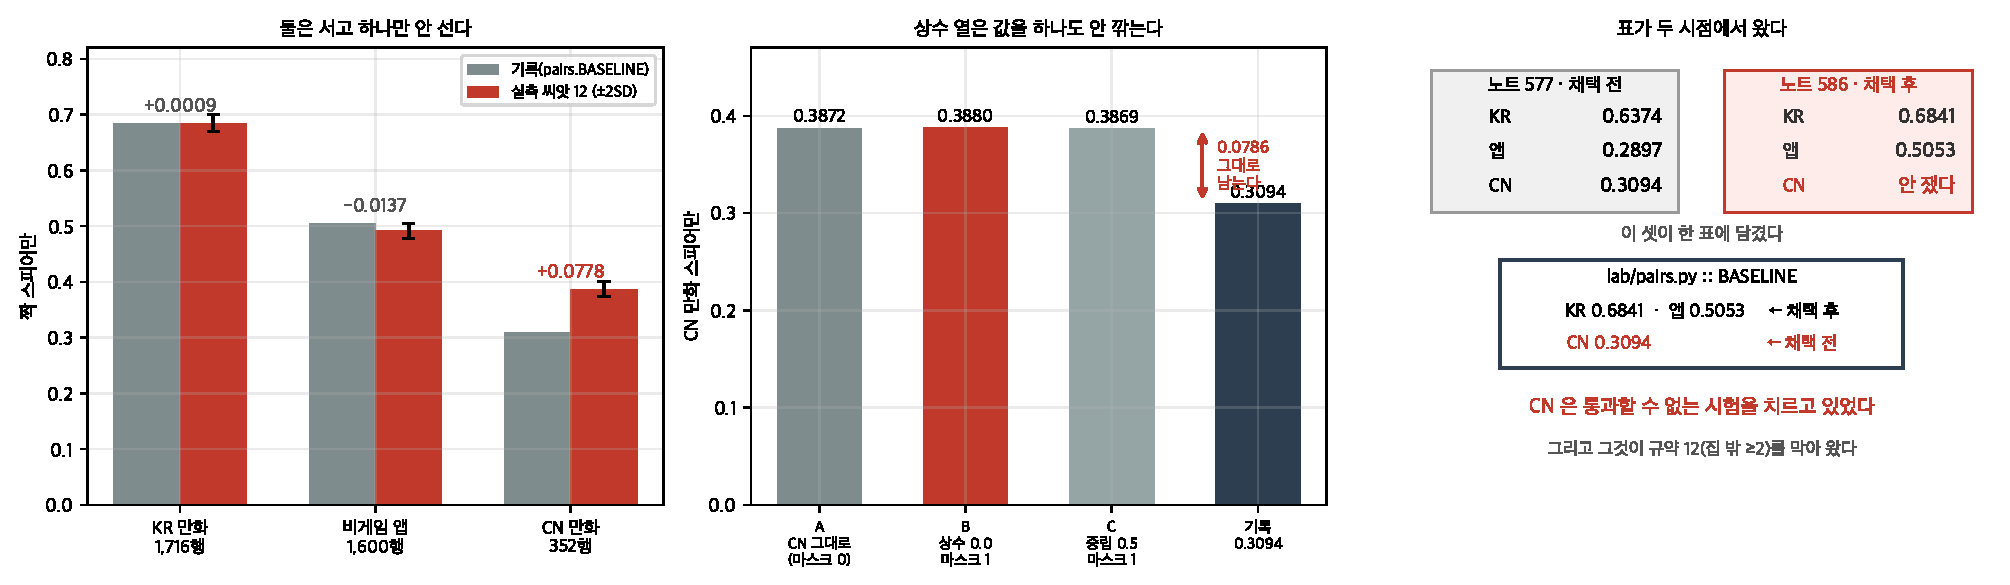
\includegraphics[width=0.99\textwidth]{figs/ruler.pdf}
\caption{왼쪽: \textbf{셋 중 둘만 선다.} 가운데: \textbf{내가 세운 기제는
기각됐다} --- 상수 열을 되넣어도 격차가 그대로다. 오른쪽: \textbf{표가 두
시점에서 왔다.}}
\end{figure}

\section{먼저 --- 씨앗도 아니고 열도 아니다}

씨앗 열둘로 세 짝을 다 쟀다(판 적합 공유).

\begin{center}
\begin{tabular}{lrrrrl}
\toprule
짝 & 실측 평균 & 씨앗 SD & 기록 & 차 & \\
\midrule
KR 만화($1{,}716$) & $0.6850$ & $0.0076$ & $0.6841$ & $\mathbf{+0.0009}$ & 선다 \\
비게임 앱($1{,}600$) & $0.4916$ & $0.0069$ & $0.5053$ & $-0.0137$ & 선다 \\
\textcolor{BrickRed}{\textbf{CN 만화}}($352$) & $0.3872$ & $0.0066$ & $0.3094$ & $\mathbf{+0.0778}$ & \textcolor{BrickRed}{\textbf{안 선다}} \\
\bottomrule
\end{tabular}
\end{center}

\textbf{씨앗 SD 가 셋 다 $0.007$ 이다} --- $352$행 $3$열인 CN 이 $1{,}716$행 $4$열인
KR 과 같다. \textbf{내 예측(CN SD $0.02{\sim}0.05$)이 틀렸다.}

\claim{\textbf{격차 $0.0778$ 은 씨앗 잡음이 아니다} --- 씨앗 폭이 $0.0216$ 인데
격차가 그 $3.6$배다. 그리고 \textbf{셋 중 둘은 선다} --- 파이프라인이 통째로
망가진 것이 아니라 CN 만의 일이다.}
{앱은 $-0.0137$ 로 씨앗 폭($0.0226$) 안에 있지만 $[$최소,최대$]$ 는 기록을 못
품는다. \textbf{경계선이다} --- 앱도 같은 병을 앓고 있을 수 있고 안 갈랐다.}

\section{내가 세운 기제는 기각됐다}

\texttt{ingest/manga\_axes.py:88} 이 \texttt{entry\_friction = 1.0 if is\_adult
else 0.0} 이고 \textbf{CN $352$행이 전부 전연령이라 값이 상수 $0.0$} 이다. 빌더가
그래서 마스크 $0$ 으로 강등한다(KR 은 값이 둘이라 산다).

\textbf{가설}: 옛 파이프라인이 그것을 강등 안 하고 마스크 $1$ 로 넣었다면, 판(JP)이
배운 \emph{전연령 가지}로 $352$행을 통째로 몰아 점수가 깎였을 것이다.
\textbf{구간 $[0.29, 0.33]$ 을 결과 보기 전에 못박았다.}

\begin{center}
\begin{tabular}{lrl}
\toprule
A. CN 그대로(마스크 $0$) & $0.3872$ & \\
\textbf{B. 상수 $0.0$ · 마스크 $1$}(옛 경로) & $\mathbf{0.3880}$ & \textcolor{BrickRed}{구간 밖} \\
C. 중립 $0.5$ · 마스크 $1$ & $0.3869$ & \\
\midrule
A$-$B & $-0.0008$ & \\
B$-$기록 & $\mathbf{+0.0786}$ & 격차가 그대로 남는다 \\
\bottomrule
\end{tabular}
\end{center}

\claim{\textbf{나는 ``모형이 그 값을 본다''와 ``모형이 그 값으로 가른다''를 섞었다.}
\textbf{트리는 값이 하나뿐인 열로는 분기를 못 만든다} --- 그래서 상수 열은 마스크가
$1$ 이든 $0$ 이든 아무 일도 안 한다($0.0008$ 차). 차원 비용조차 없다.}
{교차 확인은 예측대로였다 --- KR 의 \emph{살아 있는} \texttt{entry\_friction} 을
상수 $0.0$ 으로 누르면 $0.6850 \to 0.5573$ 이고, 이는 그냥 마스크 $0$ 으로 지운 것
($0.5663$)\textbf{보다도 낮다.} \textbf{정보를 지우는 것과 거짓을 넣는 것은 다르고,
상수를 넣는 것은 둘 다 아니다.}}

\section{진짜 원인은 대장에 있었다}

측정을 걸어 두고 대장에서 \texttt{0.3094} 를 뒤졌다.

\begin{center}
\begin{tabular}{lrrl}
\toprule
& 노트 $577$(전이) & 노트 $586$(채택 후) & \\
\midrule
KR 만화 & $0.6374$ & $0.6380 \to \mathbf{0.6841}$ & $40/40$ \\
비게임 앱 & $0.2897$ & $0.2895 \to \mathbf{0.5053}$ & $40/40$ \\
\textcolor{BrickRed}{CN 만화} & $\mathbf{0.3094}$ & \textcolor{BrickRed}{\textbf{없다 --- 안 쟀다}} & \\
\bottomrule
\end{tabular}
\end{center}

\textbf{노트 $577$ 의 전이값이 노트 $586$ 의 \emph{채택 전} 값과 소수 셋째 자리까지
같다}($0.6374$ 대 $0.6380$ · $0.2897$ 대 $0.2895$). \textbf{그리고 노트 $586$ 의
채택 목록에 CN 이 없다.}

\claim{\textbf{\texttt{BASELINE} 이 채택 전후를 섞었다.} KR·앱은 채택으로
$+0.0461$ · $+0.2157$ 올라간 값이 들어갔고 \textbf{CN 만 안 올라간 값이 남았다.}
우리 실측 격차 $+0.0778$ 이 그 둘 사이에 정확히 들어간다. \textbf{규약 $44$ 로
세웠다} --- \emph{기준선 표는 한 시점에서 와야 하고, 채택 노트가 재지 않은 자는 옛
값을 남기지 말고 \texttt{None}(안 쟀다)으로 둔다.} 빈 칸은 ``안 쟀다''를 말하고 옛
값은 ``쟀는데 이 값이다''를 말한다.}
{\textbf{이것은 아직 문서 증거이고 측정 증거가 아니다.} 결정적 시험을 등록했다
(노트 $796$) --- 채택을 되돌리면 \textbf{KR $0.6374$ · 앱 $0.2897$ · CN $0.3094$}
가 각각 $\pm 0.02$ 안에 와야 한다. \textbf{셋 다 요구한다} --- CN 하나만 맞으면
우연일 수 있다.}

\subsection*{그리고 내 실측을 기준선으로 삼지 않는다}

$0.3872$ 를 새 \texttt{BASELINE} 으로 적고 ``이제 시험 ② 통과''라고 쓰면
\textbf{자를 내 출력에 맞추고 그 자로 같은 파이프라인을 검증하는 순환}이다.
\textbf{그 조항을 측정 전에 적었다} --- \emph{원인을 이름 붙여 대고 그것이 격차를
설명해야만 기준선을 다시 적는다. 설명이 근거이고 숫자가 근거가 아니다.}

\claim{\textbf{규약 $41 \cdot 43 \cdot 44$ 는 한 병의 세 얼굴이다.} 재는 코드가
저장소에 없으면($41$) 채택 때 그 자를 안 재고, 그러면 표가 옛 값을 이고 가고($44$),
그 표를 기준선 없이 읽으면 판정이 뒤집힌다($43$). \textbf{노트 $683$ 이 이미
``다섯 자 중 넷의 채점기가 저장소에 없었다''를 적었다} --- 그 결과가 두 세션 뒤에
여기서 나왔다.}
{세 규약 모두 \textbf{이 저장소 한 곳에서 나온 관찰}이다. 다른 실험실에서도 같은
병이 도는지는 모른다.}

\section{곁가지 --- 창구 둘을 고쳤다}

사용자가 둘을 지적했다: \textbf{표가 파이프 원문으로 나간다}, \textbf{판이 자꾸 안
데워져 있다.}

\textbf{표}: \texttt{serve/static/index.html::md()} 가 손수 쓴 미니 마크다운인데
\textbf{표 문법이 아예 없었다.} 능력 카드가 표로 나가는 자리라 볼 때마다 깨졌다.
정렬까지 읽게 넣고 \textbf{여섯 경우로 검증했다}(표 · 정렬 · 표 아닌 파이프 문장 ·
구분줄 없는 줄 · 목록 뒤 표 · 표 뒤 문단).

\textbf{데우기}: \texttt{boardsvc.warm()} 이 \textbf{실측 $335$초}인데 메모리에만
둬서 \textbf{재시작할 때마다} $5$분 반을 다시 구웠다. 디스크 캐시를 붙여
$\mathbf{335\text{초} \to 0.05\text{초}}$.

\claim{\textbf{캐시의 위험은 낡는 것이고, 이 저장소는 그 병을 세 번 밟았다}(노트
$669 \cdot 672$ · \texttt{pairs.py} 가 축 파일을 일부러 저장 안 하는 이유). 그래서
\textbf{지문의 코드 목록을 적합 뒤 \texttt{sys.modules} 에서 뽑는다} --- 손으로
적으면 낡고, \texttt{lab/*.py} 를 통째로 넣으면 \texttt{lab/calib.py} 같은 무관한
파일만 고쳐도 $5$분 굽기가 날아간다. \textbf{무효화 격자 $4/4$}: 새 프로세스 적중 ·
무관 파일 적중 · 예보 경로 파일 거부 · 자료 파일 추가 거부.}
{\textbf{고치다가 조용한 실패를 내가 새로 만들었다.} \texttt{np.savez\_compressed}
는 이름이 \texttt{.npz} 로 안 끝나면 확장자를 \emph{덧붙인다} --- 임시 파일을
\texttt{...npz.tmp} 로 뒀더니 저장은 \texttt{...npz.tmp.npz} 로 되고
\texttt{os.replace} 가 없는 파일을 찾아 죽었다. \textbf{그리고 내
\texttt{except Exception: pass} 가 그것을 삼켰다} --- $335$초를 굽고도 캐시가 없는데
아무 말이 없었다. \textbf{이 저장소가 가장 자주 당하는 모양을 내가 다시 만들었다.}}

\section{남은 자리}

\textbf{규약 $12$ 는 여전히 $0/2$ 다.} 그러나 막힌 자리가 바뀌었다 --- 전에는
\emph{``CN 이 이상하다''}였고 지금은 \emph{``CN 의 자가 없다''}다.

\begin{center}
노트 $796$ 이 못박은 셋(\textbf{KR $0.6374$ · 앱 $0.2897$ · CN $0.3094$})이 서면\\
\textbf{집 밖 둘째 짝이 열리고 규약 $12$ 를 처음으로 시험할 수 있다.}
\end{center}

\end{document}
